Es gibt bereits einige Schranken mit Kennzeichenerkennung. Gerade bei Tiefgaragen, öffentlichen Parkplätzen oder Tankstellen ist die Kennzeichenerkennung eine beliebte Anwendung. Fast alle Systeme werden jedoch als Komplettset verkauft. Das heißt, es müssen die Kennzeichenerkennung sowie die Schranke gekauft werden. Bei Tankstellen dient sie hauptsächlich als Überwachungskamera.
Die Firma Taurus bietet ihren Kunden oder Kundinnen die Kennzeichenerkennung als Erweiterung an. Allerdings ist sie sehr kostspielig und nicht für den Privatgebrauch vorgesehen. Immer mehr Menschen sind auf der Suche nach einem einfacheren System für ihr Eigenheim.

\begin{figure}[H]
    \centering
    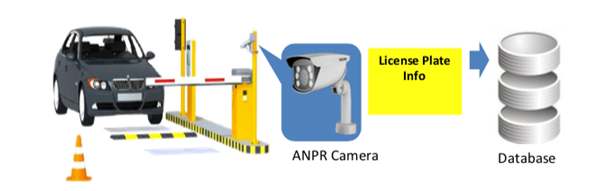
\includegraphics[width=0.8\textwidth]{pics/Taurus_Umsetzung.png}
    \caption{Umsetzung von der Firma Taurus}
    \cite{TaurusUmsetzung}
  \end{figure}

  Unsere Idee sollte kostengünstig und einfach zu montieren sein. Jedes bereits vorhandene Garagentor sollte damit erweitert werden können. Somit fallen keine Kosten für ein neues Tor an. Die Montage sollte von jedem durchgeführt werden können. Auch die Verwaltung der Kennzeichen und sonstigen Bauteile liegt in der Hand des Endverbrauchers oder der Endverbraucherin. Außerdem kann entschieden werden, welche Funktionen die Erweiterungen bieten soll. Der Kunde oder die Kundin müssen somit nicht das Komplettset kaufen. Wird eine verkleinerte Version gekauft, kann diese ganz einfach durch die verfügbaren Module erweitert werden.

  \begin{figure}[H]
    \centering
    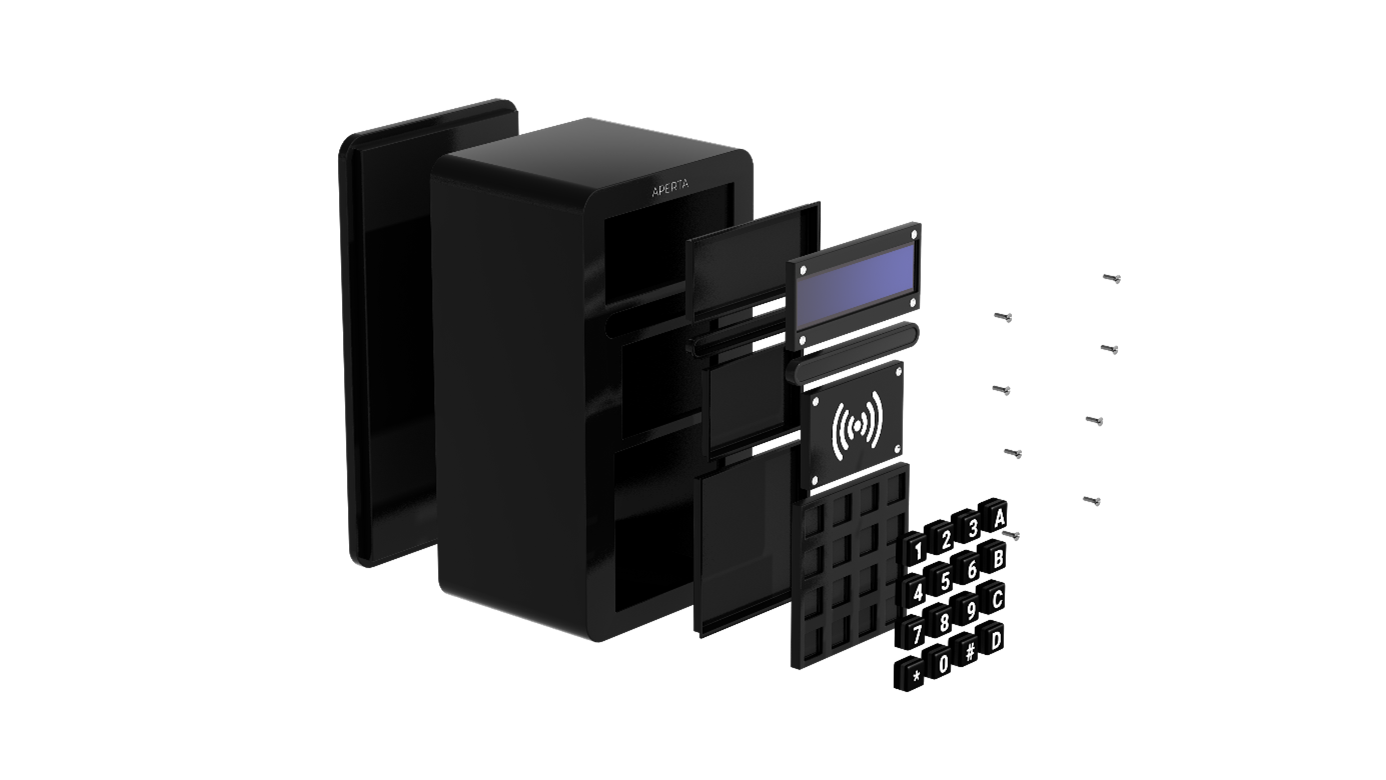
\includegraphics[width=0.8\textwidth]{pics/Modular_Aperta.png}
    \caption{Aperta zerlegt in Module}
  \end{figure}